\section{Measurement Model}
We consider the problem of recovery of a signal from its modulo measurements obtained through compressive sensing. Simply put, we aim to recover $\mathbf{x^*}\in \R^n$ from the modulo measurements $y_i=\mod(\langle \mathbf{a_i} \cdot \mathbf{x^*} \rangle,R)$ for $i = \{1,2,...,m\}$, where $\mod$ is modulo operation with respect to $R$. Typically, $m<n$. For simplicity, we assume that the modulo function operates only within two periods, one on the either side of the origin, as shown in the Fig.~\ref{fig:graph}. We construct $\mathbf{A} = \left[\mathbf{a_1~a_2~...~a_m}\right]^T$ with i.i.d. Gaussian entries. The primary assumption in our model is that the natural signal $\mathbf{x^*}$ is $s-$sparse in a chosen basis. 

\begin{figure}[h]
	\begin{center}
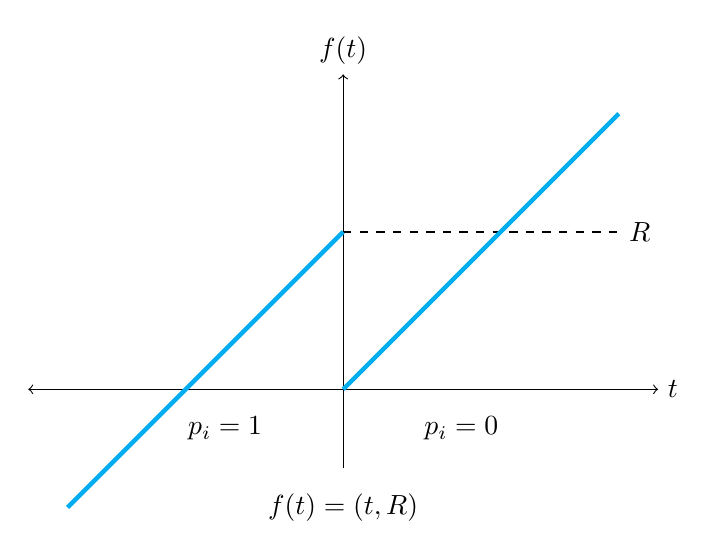
\begin{tikzpicture}
\draw[<->] (-4,0) -- (4,0) node[right] {$t$};
\draw[->] (0,-1) -- (0,4) node[above] {$f(t)$};
\draw[scale=0.5, dashed, thick] (0,4)--(7,4) node[right]{$R$};
\draw (1.5,-0.5) node(below) {$p_i = 0$};
\draw (-1.5,-0.5) node(below) {$p_i = 1$};
\draw (0,-1.5) node(right) {$f(t) = \mod(t,R)$};
\draw[scale=0.5,domain=-7:0,smooth,variable=\x,cyan, ultra thick] plot ({\x},{\x+4});
\draw[scale=0.5,domain=0:7,smooth,variable=\x,cyan, ultra thick]  plot ({\x},{\x});
\end{tikzpicture}
\end{center}
\caption{\emph{Modified modulo function for the given problem}}
\label{fig:graph}
\end{figure}

We can write the modified equation for the modulo operation under consideration as:
$$
f(t) = \mod(t,R) = t+\left( \frac{1-\sgn(t)}{2}\right)R,
$$
where $\sgn(t)$ is a signum function.

For the measurement model of the given problem, 
We define the corrected linear measurements as: 

$$
y_{c,i} =\langle \mathbf{a_i} \cdot \mathbf{x^*} \rangle.
$$

We also define the bin-index $p^*_i$ as,
$$
p^*_i = \frac{1-\sgn(\langle \mathbf{a_i} \cdot \mathbf{x^*} \rangle)}{2}.
$$
Thus,
$$
y_i = \langle \mathbf{a_i} \cdot \mathbf{x^*} \rangle + p^*_iR = y_{c,i}+p^*_iR.
$$

It is evident that if we can recover $\mathbf{p^*}$ successfully, we can calculate the correct compressed measurements $\langle \mathbf{a_i} \cdot \mathbf{x^*} \rangle$ and use them to reconstruct $\mathbf{x^*}$ with any sparse recovery algorithm such as CoSaMP.


\section{Reconstruction Algorithm}

In this section, we describe our AltMin based approach to recover $\mathbf{x^*}$ and $\mathbf{p^*}$, given $\mathbf{y, A}, s, R$. We call our algorithm MoRAM - Modulo Reconstruction using Alternative Minimization. Our approach comprises of two steps: (i) estimate initialization step, and (ii) Descent step through alternative minimization.

\subsection{Initialization}
\label{sec:init}
Similar to many non-convex techniques, MoRAM also requires an initial estimate $\mathbf{{x}^0}$ that is close to the true signal $\mathbf{{x}^*}$. The basic idea is to calculate the significant indices (or the support of $\mathbf{{x}^*}$, $S=support(\mathbf{{x}^*})$) using the suitable biased estimators, and then calculate the initial estimate using a first order biased estimator $M$ only for those significant indices contained in the support of $\mathbf{{x}^*}$. This initialization procedure is quite simple, and requires the tuning of only one parameter, the sparsity ($s$).

For support estimation, we use measurements $y_{i}$ to construct a biased estimator $L$, for which the marginal $L_{jj}$ corresponding to the $j^{th}$ element is given by:
$$
L_{jj} = \frac{1}{m}\sum_{i=1}^{m}y_{i}^2 a_{ij}^2,~~~\textnormal{for}~~~~j \in {1,...,n}.
$$
Note that the expectation $\mathbb{E}[\mathbf{L}]$ is given by,
$$
\mathbb{E}[L_{jj}] = 4x_{j}^{*2}+2R^2(1-c_1)-2R\norm{\mathbf{{x}^*}}c_2~~~~~\textnormal{where,}~c_1,c_2 \in \mathbb{R}
$$
indicating that a clear separation exists for values of expectation for $j \in S$ and $j \in S^c$, because $x_j$ is zero for $j \in S^c$ and non-zero otherwise. Therefore, we can form the approximation of the support, $\widehat{S}$ by collecting the indices of the higher magnitude elements of $\mathbb{E}[L]$. With the support known, we can throw away the columns of $\mathbf{A}$ corresponding to $j \in S^c$ for the next steps. This would make the computation faster.

Next step is to obtain the initial estimate using the first order estimator $\mathbf{M}$, defined as:
$$
M_{jj} = \frac{1}{m}\sum_{i=1}^{m}y_{i}a_{ij},~~~\textnormal{for}~~~~j \in S.
$$
To calculate $\mathbf{{x}^0}$, we use the fact that
$$
\mathbb{E}[\mathbf{M}] = \left( 1 - \sqrt{\frac{2}{\pi}}\frac{R}{2} \right) \mathbf{{x}^*}.
$$
Given enough number of samples, the sample mean of the above estimator lie very close to the expectation value. Thus, we can calculate the initial estimate $\mathbf{{x}^0}$ as:
\begin{equation}
	\mathbf{{x}^0_j} = 
	\begin{cases}
	\frac{1}{m}\sum_{i=1, j \in S}^{m}y_{i}a_{ij}~~~,& \text{if } j \in S\\
	0,              & j \in S^c.
	\end{cases}
	\label{eq:init}
\end{equation}
However, it should be noted that the quality of the initial estimate is a direct function of the number of measurements $(m)$. 


\begin{algorithm}[H]
	\caption{\textsc{MoRAM}}
	\label{alg:DMF}
	\begin{algorithmic}
		\State\textbf{Inputs:} $\mathbf{y}$, $\mathbf{A}$, $s$, $R$
		\State\textbf{Output:}  $\widehat{x}$
		\State $m,n \leftarrow \mathrm{size}(\mathbf{A})$ 
		\State $s_p \leftarrow 0.1\cdot m$
		\State \textbf{Initialization}
		\State $\mathbf{x^0} \leftarrow \textrm{Oracle}(\mathbf{y, A})$ 
		\State \textbf{Alternative Minimization}
		\For {$l =0:\mathrm{N}$}
		\State $\mathbf{{p}^{t}} \leftarrow \frac{\mathbf{1}-\sgn(\langle \mathbf{A} \cdot \mathbf{x^t} \rangle)}{2}$
		\State $\mathbf{{x}^{t+1}}\leftarrow \argmin_{[\mathbf{x~d}]^T \in \mathcal{M}_{s+s_p}}\norm{\begin{bmatrix} \mathbf{A} & \mathbf{I} \end{bmatrix} \begin{bmatrix} \mathbf{x} \\ \mathbf{d} \end{bmatrix} - \mathbf{y}}_2^2 = \cosamp(\frac{1}{\sqrt{m}}\begin{bmatrix} \mathbf{A} & \mathbf{I} \end{bmatrix},\frac{1}{\sqrt{m}}\mathbf{y},s+s_p,[\mathbf{x^t~~p^t}]^T)$
		\EndFor
	\end{algorithmic}
\end{algorithm}

\subsection{Alternative Minimization}
\label{sec:altmin}

Using Eq.~\ref{eq:init}, we calculate the initial estimate of the signal $\mathbf{{x}^0}$ which is relatively close to the true vector $\mathbf{x^*}$. Starting with $\mathbf{{x}^0}$, we  calculate the estimates $\mathbf{p}$ and $\mathbf{x}$ in alternating fashion to converge to the original signal $\mathbf{x^*}$. At each iteration of our Alternative Minimization, we use the current estimate of the signal ${\mathbf{x^t}}$ to get the value of the bin-index vector $\mathbf{{p}^t}$ as following:
\begin{equation}
\mathbf{{p}^{t}} = \frac{\mathbf{1}-\sgn(\langle \mathbf{A} \cdot \mathbf{x^t} \rangle)}{2}.
\label{step1}
\end{equation}

 
 Given $\mathbf{x^0}$ is close to $\mathbf{x^*}$, $\mathbf{p^0}$ would also be close to $\mathbf{p^*}$. Ideal way is to calculate the correct compressed measurements $\mathbf{y^t_c}$ using $\mathbf{p^t}$, and use $\mathbf{y_c}$ with CoSaMP to calculate the next estimate $\mathbf{{x}_{t+1}}$. Thus,


$$
\mathbf{y^t_c} = \langle \mathbf{A}\mathbf{x_{t}} \rangle = \mathbf{y} - \mathbf{p^t}R,
$$
$$
\mathbf{{x}^{t+1}} = \argmin_{\mathbf{x} \in \mathcal{M}_s}\norm{\mathbf{Ax} - \mathbf{y^t_c}}_2^2, %~~\mathrm{s.to}~~x^* \in \mathcal{M}_s,
$$

\begin{equation}
\implies \mathbf{{x}^{t+1}} = \cosamp(\frac{1}{\sqrt{m}}\mathbf{A},\frac{1}{\sqrt{m}}\mathbf{y^t_c},s,\mathbf{x_t}).
\label{eq:cosamp}
\end{equation}


 However, it should be noted that even the small error $\mathbf{d} = \mathbf{p^t - p^*}$ would reflect heavily in the calculation of $\mathbf{y^t_c}$, as each incorrect bin-index would add a noise of the magnitude $R$ in $\mathbf{y^t_c}$. Experiments suggest that the CoSaMP is not robust enough to cope up with such large errors in $\mathbf{y^t_c}$. To tackle this issue, we augmented the sparse recovery problem using the fact that the nature of error $\mathbf{d^t_p}$ is sparse; and each erroneous element of $\mathbf{p}$ adds a noise of the magnitude $R$ in $\mathbf{y^t_c}$. We take the sparsity of $\mathbf{d^t}$ to be $s_p = 0.1\times m$, suggesting that at most the $10\%$ of the total elements are classified with wrong bin-indices.
 
 The augmented optimization problem becomes,
  
$$
\mathbf{{x}^{t+1}}=\argmin_{[\mathbf{x~d}]^T \in \mathcal{M}_{s+s_p}}\norm{\begin{bmatrix} \mathbf{A} & \mathbf{I} \end{bmatrix} \begin{bmatrix} \mathbf{x} \\ \mathbf{d} \end{bmatrix} - \mathbf{y}}_2^2, %~~\mathrm{s.to}~~x^* \in \mathcal{M}_s,
$$
\begin{equation}
\implies \mathbf{{x^{t+1}}} = \cosamp(\frac{1}{\sqrt{m}}\begin{bmatrix} \mathbf{A} & \mathbf{I} \end{bmatrix},\frac{1}{\sqrt{m}}\mathbf{y},s+s_p,[\mathbf{x^t~~p^t}]^T).
\label{eq:robcosamp}
\end{equation}
We call the step in Eq.~\ref{eq:robcosamp} a Robust CoSaMP. 

We repeat the steps of bin index calculation (as in Eq.~\ref{step1}) and sparse recovery (as in Eq.~\ref{eq:cosamp} or Eq.~\ref{eq:robcosamp}) alternatively for $\mathrm{N}$ iterations. While the sparse recovery with robust CoSaMP (Eq.~\ref{eq:robcosamp}) improves the reconstruction performance for large values of $R$ by making the sparse recovery step less susceptible to the errors, CoSaMP can also used in its original form (as in Eq.~\ref{eq:cosamp}) for lower values of $R$.

Thus, we can have two variants of the MoRAM algorithm: (i)MoRAM with CoSaMP, and (ii) MoRAM with robust CoSaMP. 

%$$
%\norm{\begin{bmatrix} \mathbf{A} & \mathbf{I} \end{bmatrix} \begin{bmatrix} \mathbf{x^*} \\ \mathbf{d} \end{bmatrix} - \mathbf{y}}_2^2.
%$$

%


\subsection{Experiments}

\subsubsection{Analyzing sensitivity towards the initial estimate}
For this experiment, we use a synthetic signal generated randomly with $n=1000$ and $s=20$. 
Our aim is to analyze the sensitivity of our algorithm towards the initial estimate $\mathbf{x^0}$. %Currently, in the absence of a suitable initialization method, 
For that, we compute the initial estimate $\mathbf{x^0}$ by adding a Gaussian noise to the original signal. In Fig.~\ref{fig:pl}, we plot the variation of the relative reconstruction error ($\frac{\norm{\mathbf{x^*-x^N}}}{\norm{\mathbf{x^*}}}$) with the relative error in initial estimate ($\frac{\norm{\mathbf{x^*-x^0}}}{\norm{\mathbf{x^*}}}$). We plot the similar curves for different values of number of measurements $m$.
\begin{figure}[t]
	\begin{center}
		%\vspace{-0em}
		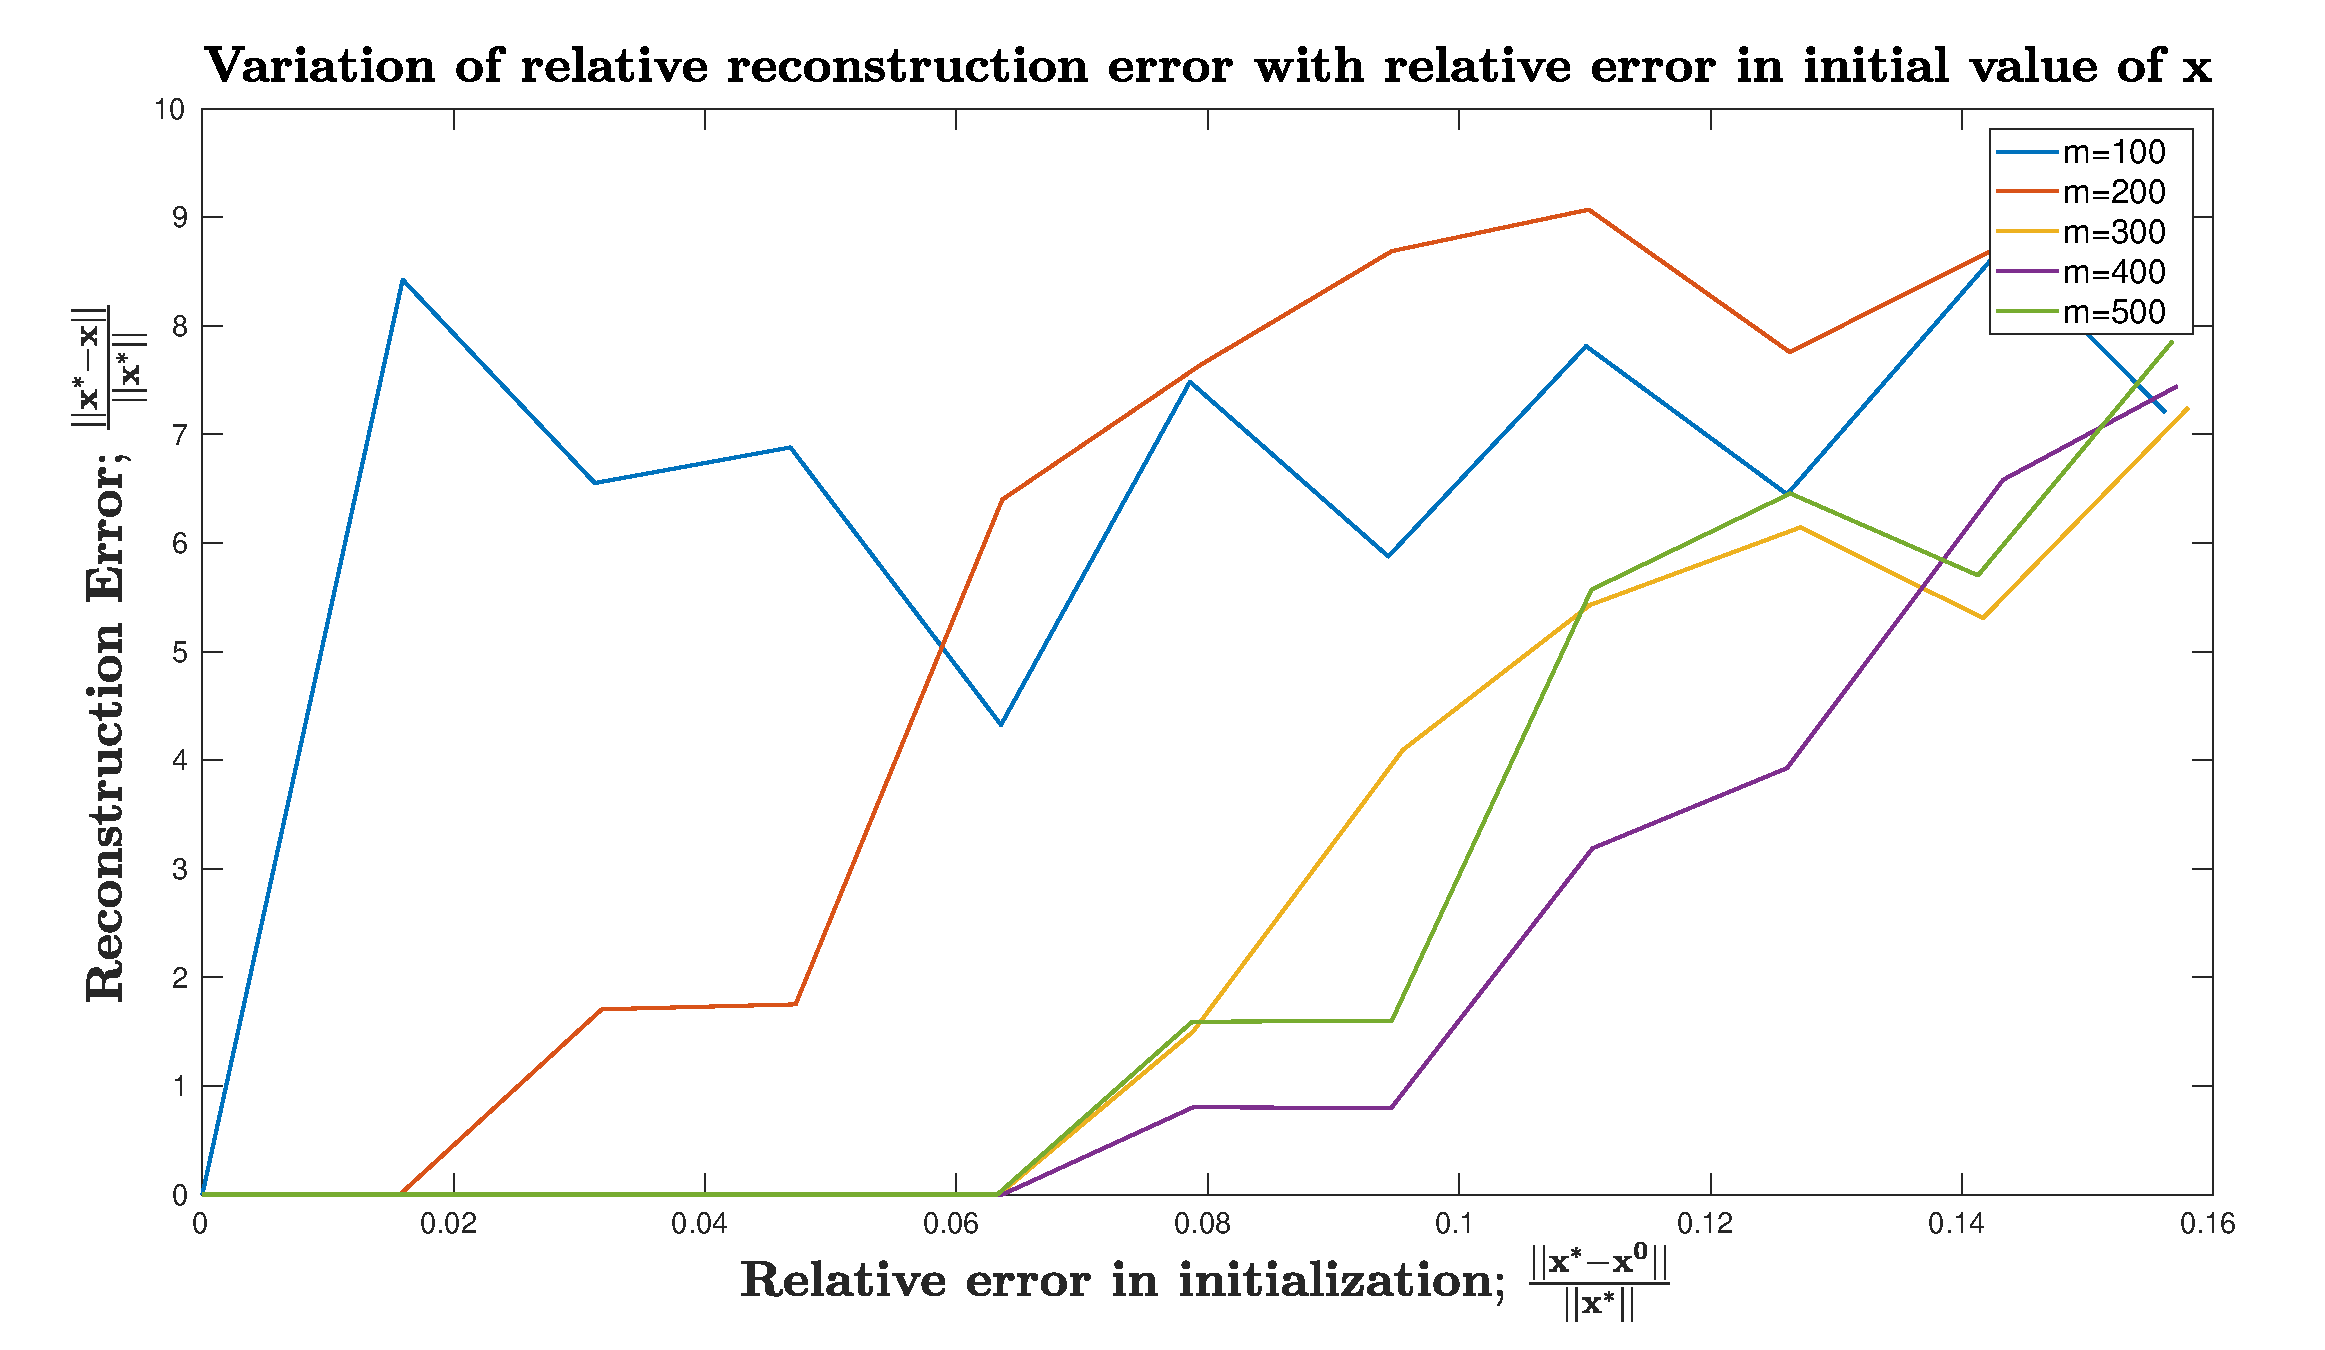
\includegraphics[width=\linewidth]{./fig/graph.pdf}
	\end{center}
	\caption{}
	\label{fig:pl}
\end{figure}

%\newpage
%\begin{section}{Appendix}
%\begin{figure}[t]
%	\begin{center}
%		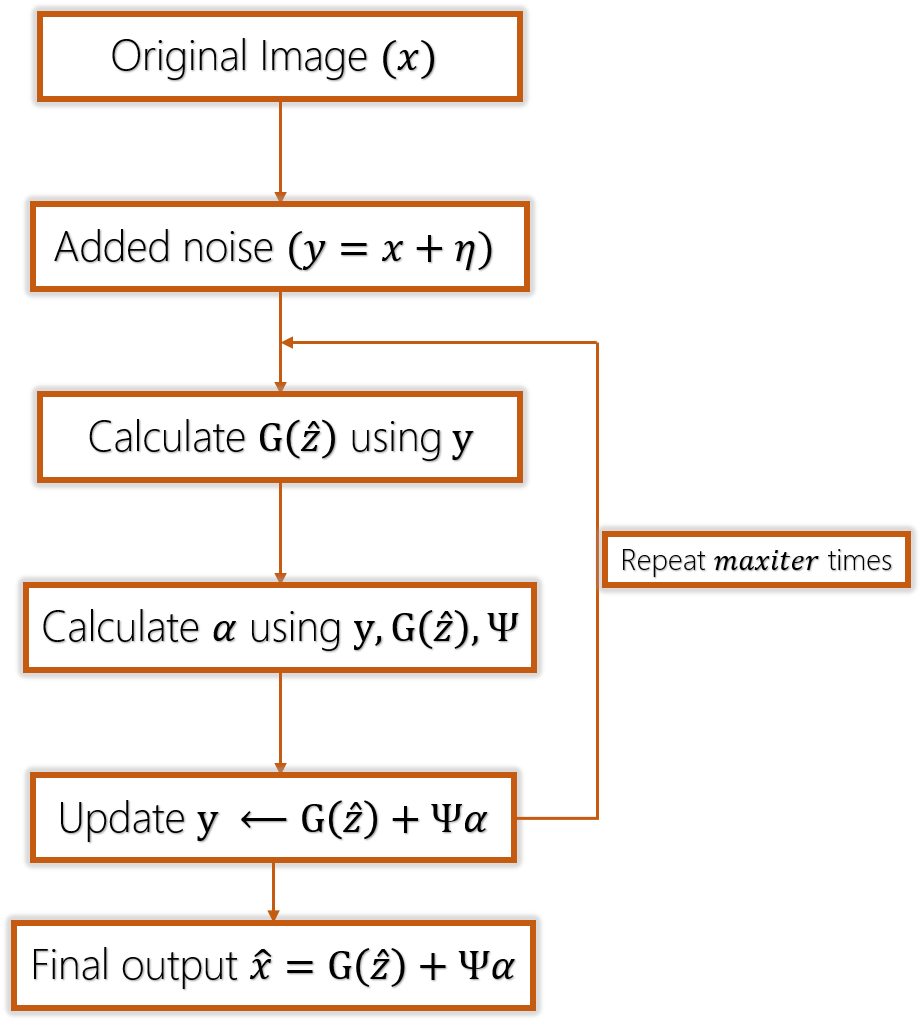
\includegraphics[width=0.4\linewidth]{./fig/alg.png}
%	\end{center}
%	\caption{\emph{Our approach}}
%	\label{fig:alg}
%\end{figure}
%\end{section}

\subsubsection{Performance of our algorithm for signal reconstruction}
We perform experiments on a synthetic signal generated randomly with $n=1000$ and $s=5$. We compute the initial estimate $\mathbf{x^0}$ using first order estimator method described in~\ref{sec:init}. we plot the variation of the relative reconstruction error ($\frac{\norm{\mathbf{x^*-x^N}}}{\norm{\mathbf{x^*}}}$) with number of measurements $m$ for both the variants of sparse recovery algorithm as described in~\ref{sec:altmin}.

It is important to note that unlike the absolute value function, the modulo function described in Fig.~\ref{fig:graph} is not scale-invariant. The modulo function works over the quantities $y_{c,i}=\langle \mathbf{a_i} \cdot \mathbf{x^*} \rangle, i=1,..,m$; and it is defined over the parameter $R$; thus depending on the magnitudes of $y_{c,i}$ and $R$ relative to each other, the behavior of the measurement model and the reconstruction algorithm would be altered. For instance, if the value of $R$ is too small compared to the range of the $y_{c,i}$, the modulo operation would hardly have any effect on the measurements, leaving $\mathbf{y_c \approx y}$. To analyze such variations, we fix the $R =1$ in our experiments, while varying the signal strength to vary the magnitudes of $y_{c,i}$. We measure the signal strength by the norm of the original signal ($\norm{\mathbf{{x}^*}}=1$).

Another important factor affecting the reconstruction is the quality of the initial estimate ($\mathbf{{x}^0}$) obtained through first order estimation. As described in~\ref{sec:init}, the quality of the initial estimate is a direct function of number of measurements ($m$). As we set $m$ higher, the initial estimate $\mathbf{{x}^0}$ would move closer to the original signal $\mathbf{{x}^*}$. For our experiments, we consider two ranges of $m$: $m \in [100,1000]$ and $m \in [1000,10000]$.
\begin{center}
	\begin{table}
		\centering
		\begin{tabular}{cccc}\toprule
			\multicolumn{4}{c}{\small{\textbf{Fixed:} $R=1, n=1000, s=5$}} \\ \midrule
			\multicolumn{2}{c}{\textbf{CoSaMP}}&\multicolumn{2}{c}{\textbf{robust CoSaMP}}
			\\\cmidrule(r){1-2}\cmidrule(r){3-4}  
			\small{$\norm{\mathbf{{x}^*}}=1$}&\small{$\norm{\mathbf{{x}^*}}=0.5$}&\small{$\norm{\mathbf{{x}^*}}=1$}&\small{$\norm{\mathbf{{x}^*}}=0.5$}\\\midrule
			\hyperref[fig:plot-1-1]{Figure~\ref{fig:plot-1-1}} & \hyperref[fig:plot-1-2]{Figure~\ref{fig:plot-1-2}}
			& \hyperref[fig:plot-1-3]{Figure~\ref{fig:plot-1-3}}  & \hyperref[fig:plot-1-4]{Figure~\ref{fig:plot-1-4}} \\
			\bottomrule
		\end{tabular}
		\caption{The Results}\label{Tab2}
	\end{table} 	
\end{center}
In the Table~\ref{Tab2}, we provide experimental results for each of the combination above.

 
\begin{figure}[t]
	\begin{center}
		%\vspace{-0em}
		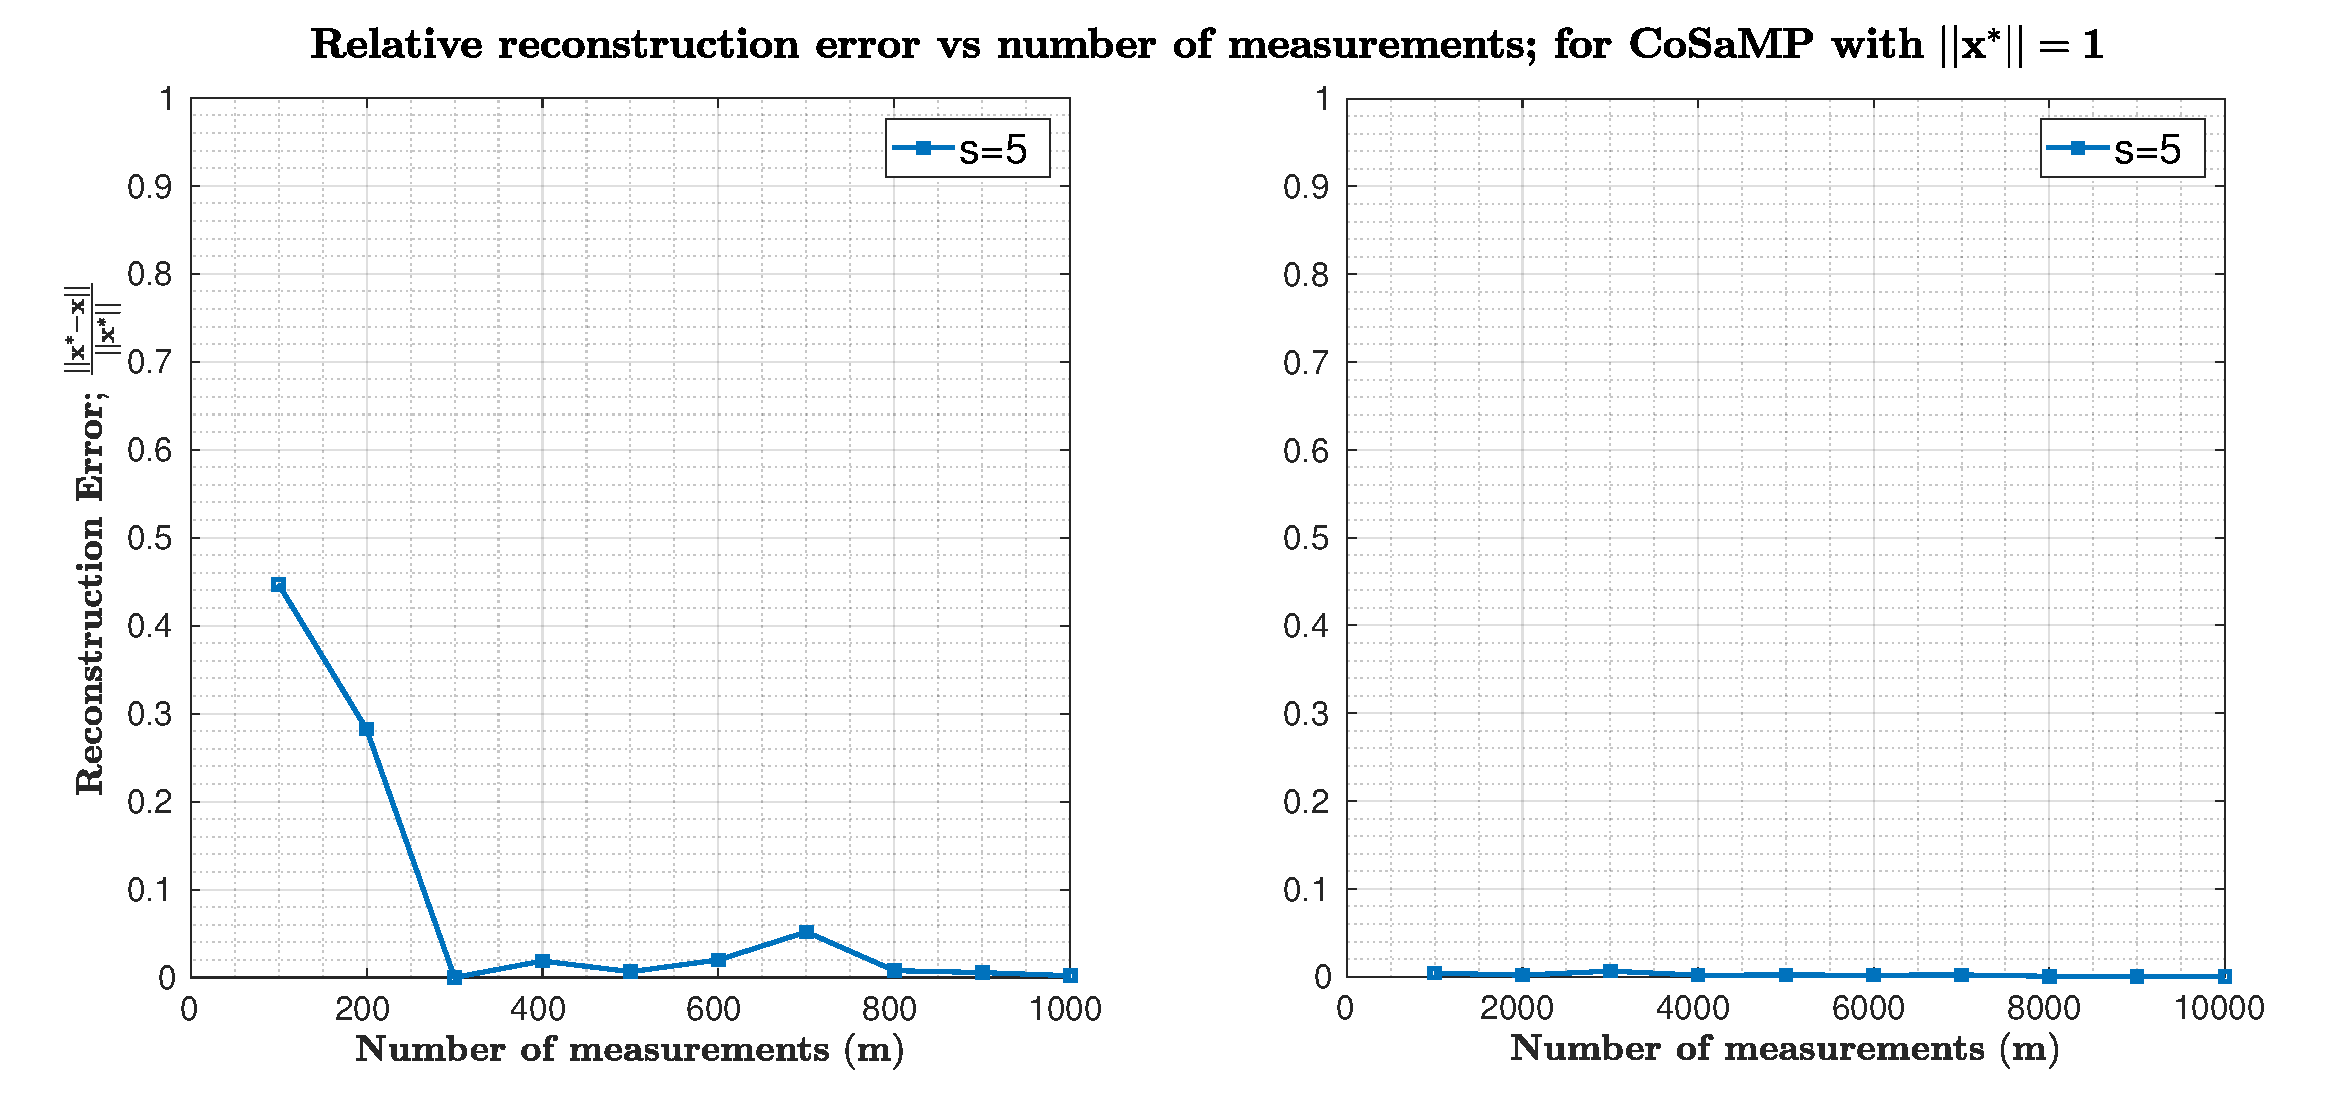
\includegraphics[width=\linewidth]{./fig/plot-1-1.pdf}
	\end{center}
	\caption{}
	\label{fig:plot-1-1}
\end{figure}

\begin{figure}[t]
	\begin{center}
		%\vspace{-0em}
		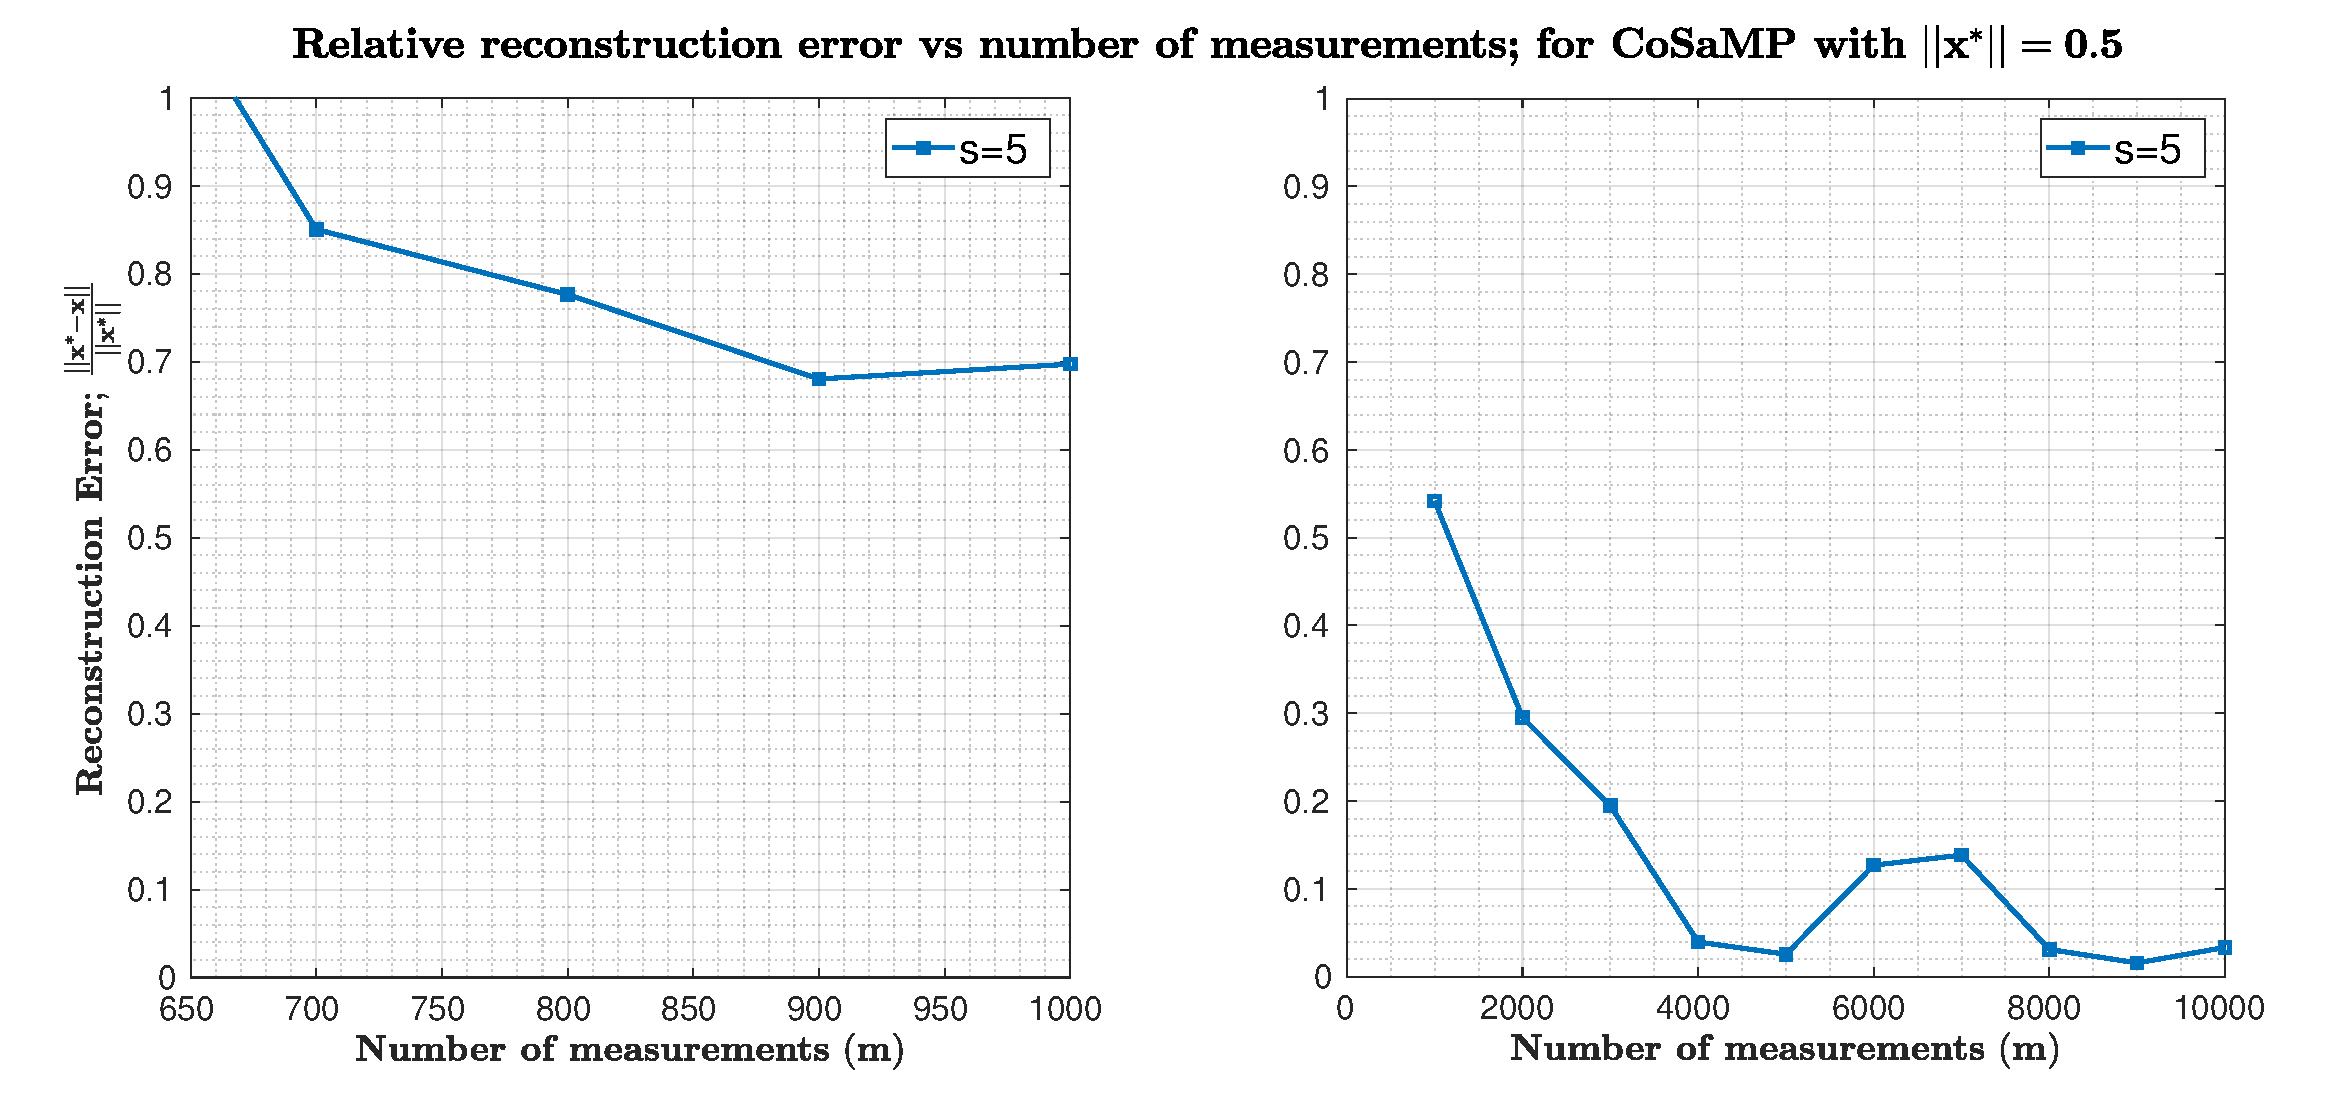
\includegraphics[width=\linewidth]{./fig/plot-1-2.pdf}
	\end{center}
	\caption{}
	\label{fig:plot-1-2}
\end{figure}
%
\begin{figure}[t]
	\begin{center}
		%\vspace{-0em}
		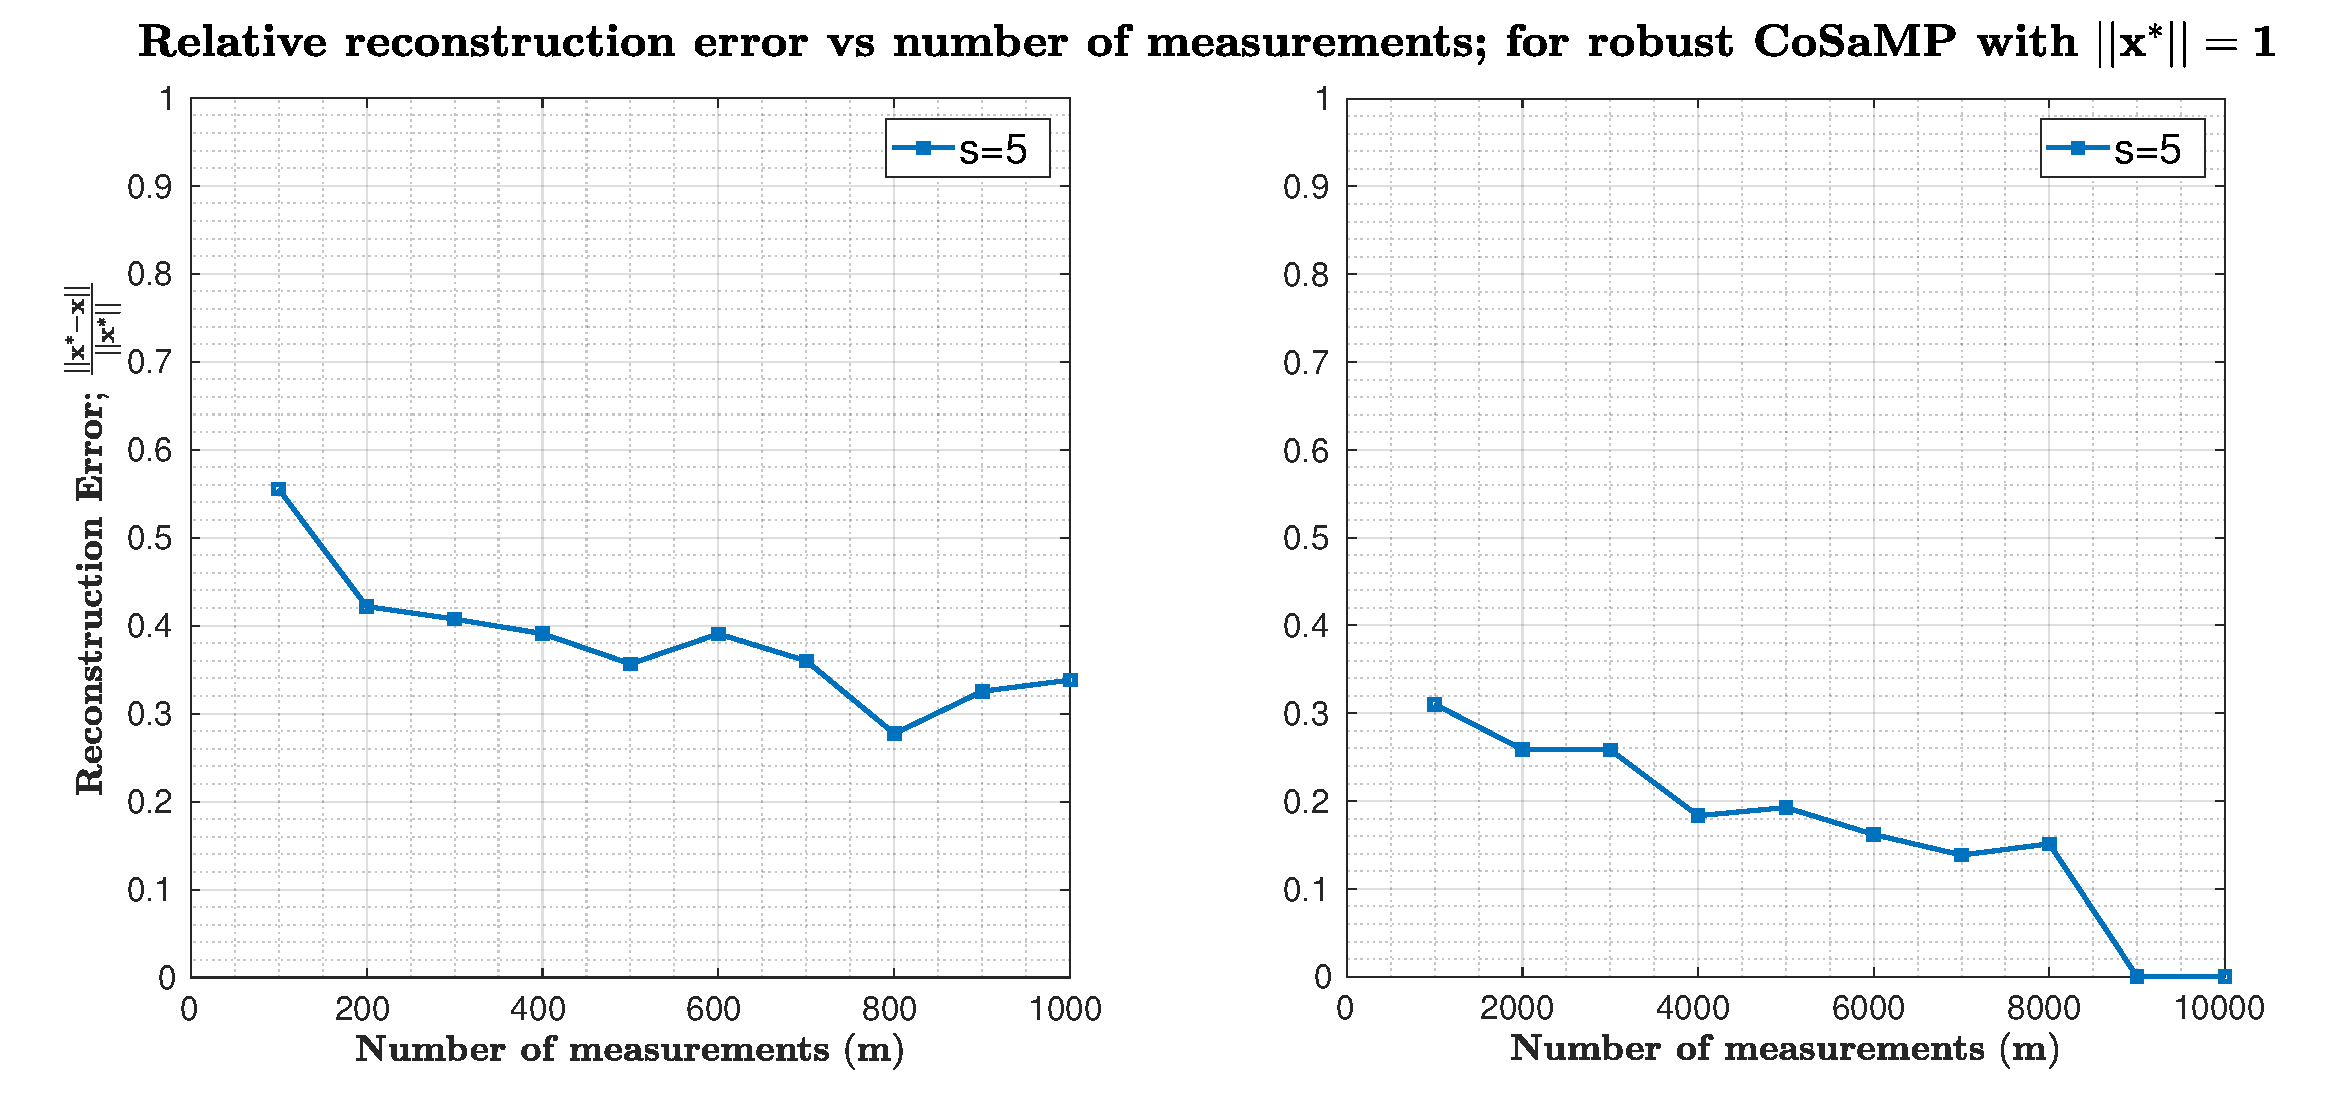
\includegraphics[width=\linewidth]{./fig/plot-1-3.pdf}
	\end{center}
	\caption{}
	\label{fig:plot-1-3}
\end{figure}
%
\begin{figure}[t]
	\begin{center}
		%\vspace{-0em}
		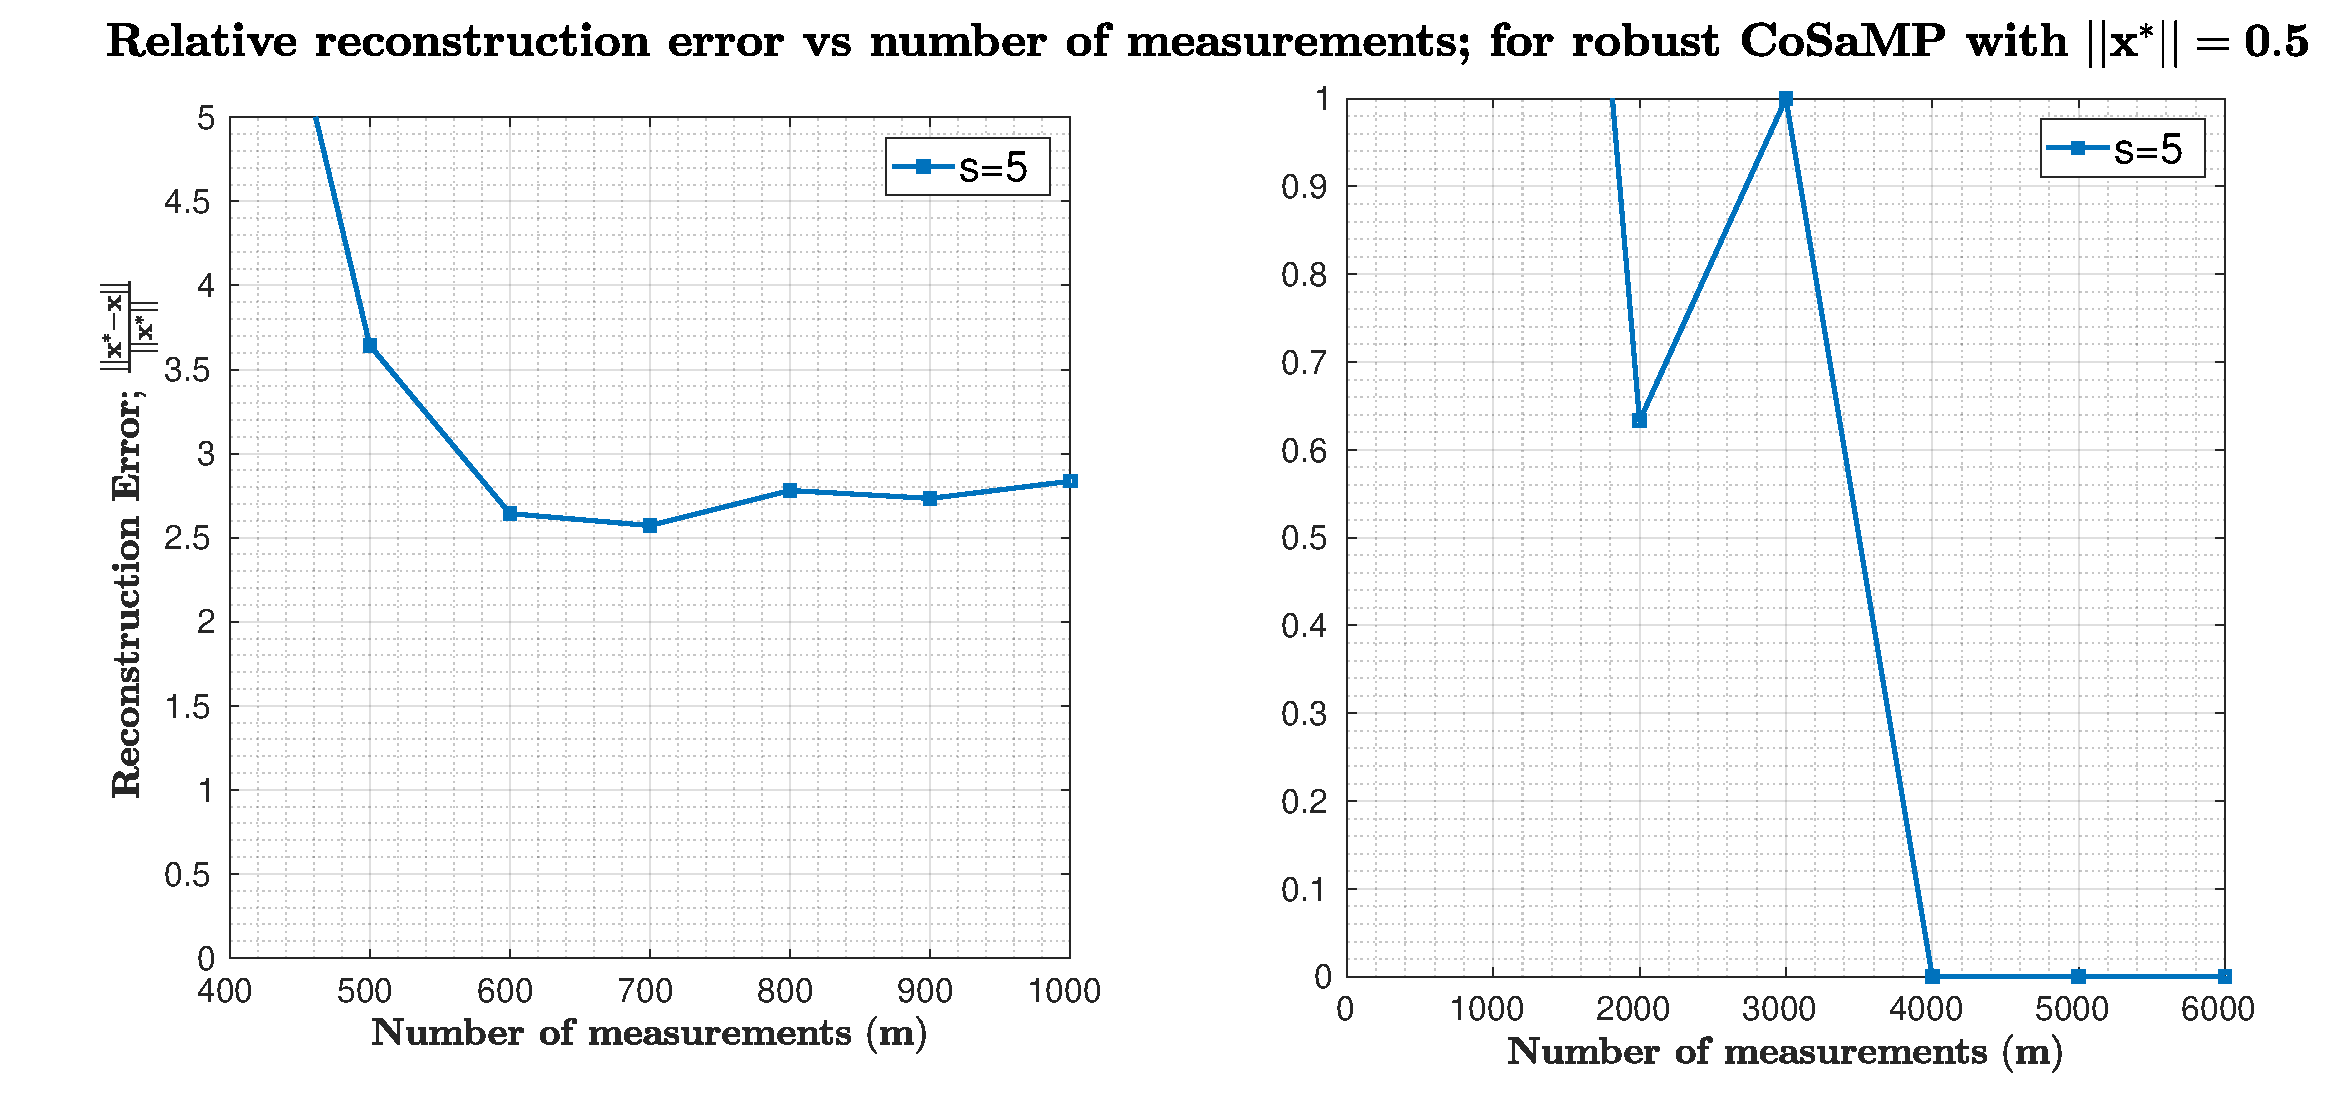
\includegraphics[width=\linewidth]{./fig/plot-1-4.pdf}
	\end{center}
	\caption{}
	\label{fig:plot-1-4}
\end{figure}